\section{eo\-Vl\-Del\-Mutation$<$ EOT $>$ Class Template Reference}
\label{classeo_vl_del_mutation}\index{eoVlDelMutation@{eoVlDelMutation}}
Deletion of a gene By default at a random position, but a \char`\"{}chooser\char`\"{} can be specified can of course be applied to both order-dependent and order-independent.  


{\tt \#include $<$eo\-Variable\-Length\-Mutation.h$>$}

Inheritance diagram for eo\-Vl\-Del\-Mutation$<$ EOT $>$::\begin{figure}[H]
\begin{center}
\leavevmode
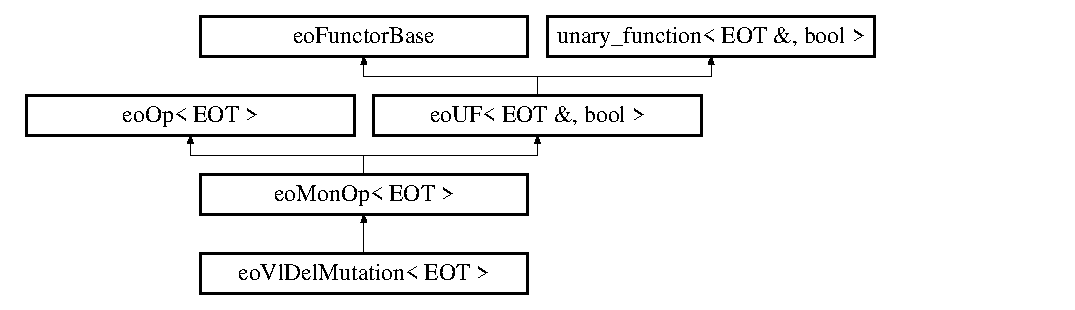
\includegraphics[height=3.71476cm]{classeo_vl_del_mutation}
\end{center}
\end{figure}
\subsection*{Public Types}
\begin{CompactItemize}
\item 
typedef EOT::Atom\-Type {\bf Atom\-Type}\label{classeo_vl_del_mutation_w0}

\end{CompactItemize}
\subsection*{Public Member Functions}
\begin{CompactItemize}
\item 
{\bf eo\-Vl\-Del\-Mutation} (unsigned \_\-n\-Min, {\bf eo\-Gene\-Del\-Chooser}$<$ {\bf EOT} $>$ \&\_\-chooser)
\begin{CompactList}\small\item\em ctor with an external gene chooser \item\end{CompactList}\item 
{\bf eo\-Vl\-Del\-Mutation} (unsigned \_\-n\-Min)
\begin{CompactList}\small\item\em ctor with uniform gene chooser - the default \item\end{CompactList}\item 
bool {\bf operator()} ({\bf EOT} \&\_\-eo)
\begin{CompactList}\small\item\em Do the job (delete one gene). \item\end{CompactList}\item 
virtual std::string {\bf class\-Name} () const \label{classeo_vl_del_mutation_a3}

\end{CompactItemize}
\subsection*{Private Attributes}
\begin{CompactItemize}
\item 
unsigned {\bf n\-Min}\label{classeo_vl_del_mutation_r0}

\item 
{\bf eo\-Uniform\-Gene\-Chooser}$<$ {\bf EOT} $>$ {\bf u\-Chooser}\label{classeo_vl_del_mutation_r1}

\item 
{\bf eo\-Gene\-Del\-Chooser}$<$ {\bf EOT} $>$ \& {\bf chooser}\label{classeo_vl_del_mutation_r2}

\end{CompactItemize}


\subsection{Detailed Description}
\subsubsection*{template$<$class EOT$>$ class eo\-Vl\-Del\-Mutation$<$ EOT $>$}

Deletion of a gene By default at a random position, but a \char`\"{}chooser\char`\"{} can be specified can of course be applied to both order-dependent and order-independent. 



Definition at line 110 of file eo\-Variable\-Length\-Mutation.h.

\subsection{Constructor \& Destructor Documentation}
\index{eoVlDelMutation@{eo\-Vl\-Del\-Mutation}!eoVlDelMutation@{eoVlDelMutation}}
\index{eoVlDelMutation@{eoVlDelMutation}!eoVlDelMutation@{eo\-Vl\-Del\-Mutation}}
\subsubsection{\setlength{\rightskip}{0pt plus 5cm}template$<$class EOT$>$ {\bf eo\-Vl\-Del\-Mutation}$<$ {\bf EOT} $>$::{\bf eo\-Vl\-Del\-Mutation} (unsigned {\em \_\-n\-Min}, {\bf eo\-Gene\-Del\-Chooser}$<$ {\bf EOT} $>$ \& {\em \_\-chooser})\hspace{0.3cm}{\tt  [inline]}}\label{classeo_vl_del_mutation_a0}


ctor with an external gene chooser 

\begin{Desc}
\item[Parameters:]
\begin{description}
\item[{\em n\-Min}]min number of atoms to leave in the individual \item[{\em \_\-gene\-Chooser}]an eo\-Gene\-CHooser to choose which one to delete \end{description}
\end{Desc}


Definition at line 121 of file eo\-Variable\-Length\-Mutation.h.\index{eoVlDelMutation@{eo\-Vl\-Del\-Mutation}!eoVlDelMutation@{eoVlDelMutation}}
\index{eoVlDelMutation@{eoVlDelMutation}!eoVlDelMutation@{eo\-Vl\-Del\-Mutation}}
\subsubsection{\setlength{\rightskip}{0pt plus 5cm}template$<$class EOT$>$ {\bf eo\-Vl\-Del\-Mutation}$<$ {\bf EOT} $>$::{\bf eo\-Vl\-Del\-Mutation} (unsigned {\em \_\-n\-Min})\hspace{0.3cm}{\tt  [inline]}}\label{classeo_vl_del_mutation_a1}


ctor with uniform gene chooser - the default 

\begin{Desc}
\item[Parameters:]
\begin{description}
\item[{\em n\-Min}]min number of atoms to leave in the individual \end{description}
\end{Desc}


Definition at line 128 of file eo\-Variable\-Length\-Mutation.h.

\subsection{Member Function Documentation}
\index{eoVlDelMutation@{eo\-Vl\-Del\-Mutation}!operator()@{operator()}}
\index{operator()@{operator()}!eoVlDelMutation@{eo\-Vl\-Del\-Mutation}}
\subsubsection{\setlength{\rightskip}{0pt plus 5cm}template$<$class EOT$>$ bool {\bf eo\-Vl\-Del\-Mutation}$<$ {\bf EOT} $>$::operator() ({\bf EOT} \& {\em \_\-eo})\hspace{0.3cm}{\tt  [inline, virtual]}}\label{classeo_vl_del_mutation_a2}


Do the job (delete one gene). 

\begin{Desc}
\item[Parameters:]
\begin{description}
\item[{\em \_\-eo}]the {\bf EO}{\rm (p.\,\pageref{class_e_o})} to mutate \end{description}
\end{Desc}


Implements {\bf eo\-UF$<$ EOT \&, bool $>$} {\rm (p.\,\pageref{classeo_u_f_a1})}.

Definition at line 134 of file eo\-Variable\-Length\-Mutation.h.

The documentation for this class was generated from the following file:\begin{CompactItemize}
\item 
eo\-Variable\-Length\-Mutation.h\end{CompactItemize}
